\subsection{Regularization and variable selection}

In this section, we apply thee of the previously discussed prior distributions to Linear and Logistic regression.

We create a synthetic data sets (consisting of training and test data) from each of two different setting, referred to as scenario A and B.

\begin{itemize}
    \item \textbf{Scenario A}: a well-behaved scenario without collinearity to examine shrinkage:
    \begin{equation*}
        \begin{aligned}
            &n = 150,\; n_{train} = 100,\;n_{test} = 50 \\
            &\btheta = (2, 1.5, 0, 0, 0) \\
            &\bX \sim \Ncal(\bnull, \bI) \\
            &\text{linear: } \by \mid \btheta \sim \Ncal(\bX \btheta,\bI)\quad \text{logistic: } \by \sim \text{Ber}(\sigma(\bX \btheta))
        \end{aligned}
    \end{equation*}
    \item \textbf{Scenario B}: a low-information scenario where $n \approx p$ with collinearity between informative and non-informative covariates:
    \begin{equation*}
        \begin{aligned}
            &n = 150,\; n_{train} = 30,\;n_{test} = 120 \\
            &\btheta = (2, 1.5, 0, \overset{26\; \text{times}}{\dots}, 0) \\
            &\bX \sim \Ncal(\bnull, \Sd), \quad \Sd =
                    \begin{pmatrix}
                    1 &        &         &        &        \\
                        & \!\!S_3\!\! &        & 0      &        \\
                        &        & I_{26} &        &        \\
                        & 0      &        &        &        \\
                    \end{pmatrix},
                    \qquad
                    S_3 = 
                    \begin{pmatrix}
                    1   & 0.8 & 0.8\\
                    0.8 & 1   & 0.8\\
                    0.8 & 0.8 & 1
                    \end{pmatrix}\\
            &\text{linear: } \by \mid \btheta \sim \Ncal(\bX \btheta, \bI)\quad \text{logistic: } \by \sim \text{Ber}(\sigma(\bX \btheta))
        \end{aligned}
    \end{equation*}
\end{itemize}

For each scenario, we fit three linear and logistic regression models.
We set the Markov chain length as 20000, a burnin period of 1000 and a thinning interval of 10. We used three different prior distributions: A flat prior as a benchmark, using the conjugate setting described in \autoref{eq:flat-prior} with the R-package \texttt{brms}.
The Gaussian prior variance was set to $10^6$ and for the Gamma prior we set $a = 0.001, b=0.001$ which results in an uninformative prior. To examine regularization, we used a Ridge prior (see \autoref{eq:ridge}) and a Lasso prior (see \autoref{eq:lasso})  with the \texttt{bayesreg} package and automatic optimization of the regularization parameters $\tau^2$ and $\lambda^2$.\\

Since Ridge and Lasso regularization cannot perform variable selection, we included the coefficients based on the Bayesian credibility interval criterion described in \citet{van_erp_shrinkage_2019}.
We were interested in whether the models could accurately select relevant variables (1), and in the correct prediction of the outcome $\by$ (2).\\

To evaluate (1), we calculated correctly identified influential coefficients (Hits) and the falsely as influential declared coefficients (FP)
For evaluation of predictive accuracy (2), we used the test data to calculate the mean (or: expected) log predictive posterior density (MLPPD), which was proposed by \citet{gelman_understanding_2013} and used for similar purposes by \citet{van_erp_shrinkage_2019}. Since the log-likelihood is a proper scoring rule, it is well-suited to evaluate Bayesian regression models.
Results for these metrics can be seen in \autoref{tab:reg_AB}.
In \autoref{fig:reg-params}, we assessed the uncertainty of the model parameter estimates.


\begin{table}[ht]
    \centering
    \begin{tabular}{@{} ll  rrr   rrr @{}}
        \toprule
        Model & Prior 
            & \multicolumn{3}{c}{Scenario A} 
            & \multicolumn{3}{c}{Scenario B} \\
        \cmidrule(lr){3-5} \cmidrule(lr){6-8}
                &      
            & Hits (of 2) & FP (of 3)  & MLPPD      
            & Hits (of 2) & FP (of 28) & MLPPD     \\
        \midrule
        %---- Linear block
        Linear & flat   & 2 &  0 & -1.425  
        & 2 &  1 &   -1.605     \\
        Linear & lasso  & 2 &  0 & -1.424  
                & 2 &  0 &   -1.464     \\
        Linear & ridge  & 2 &  0 & -1.427  
                & 2 &  0 &   -1.575     \\
        \specialrule{1.5pt}{0pt}{0pt}
        %---- Logit block
        Logit  & flat   & 2 &  1 & -0.390  
        & 0 & 21 &   $-\infty$  \\
        Logit  & lasso  & 1 &  0 & -0.463  
        & 1 &  0 &   -0.485     \\
        Logit  & ridge  & 1 &  0 & -0.455  
        & 1 &  0 &   -0.493     \\
        \bottomrule
    \end{tabular}
    \caption{Evaluation under scenario A and B. Linear Regression regardless of prior identified influential coefficients more accurately (Hits) and misclassified less coefficients as influential (FP). We see the effect of regularization more strongly in Logistic regression, where regardless of the scenario, less coefficients were declared influential. Regularization priors performed better in the non-informative scenario B. Except for the flat prior, Bayesian logistic regression made more accurate predictions than linear regression, but the MLPPD is not very different between regularization and no regularization.}
    \label{tab:reg_AB}
\end{table}

\begin{figure}[htbp]
    \centering
    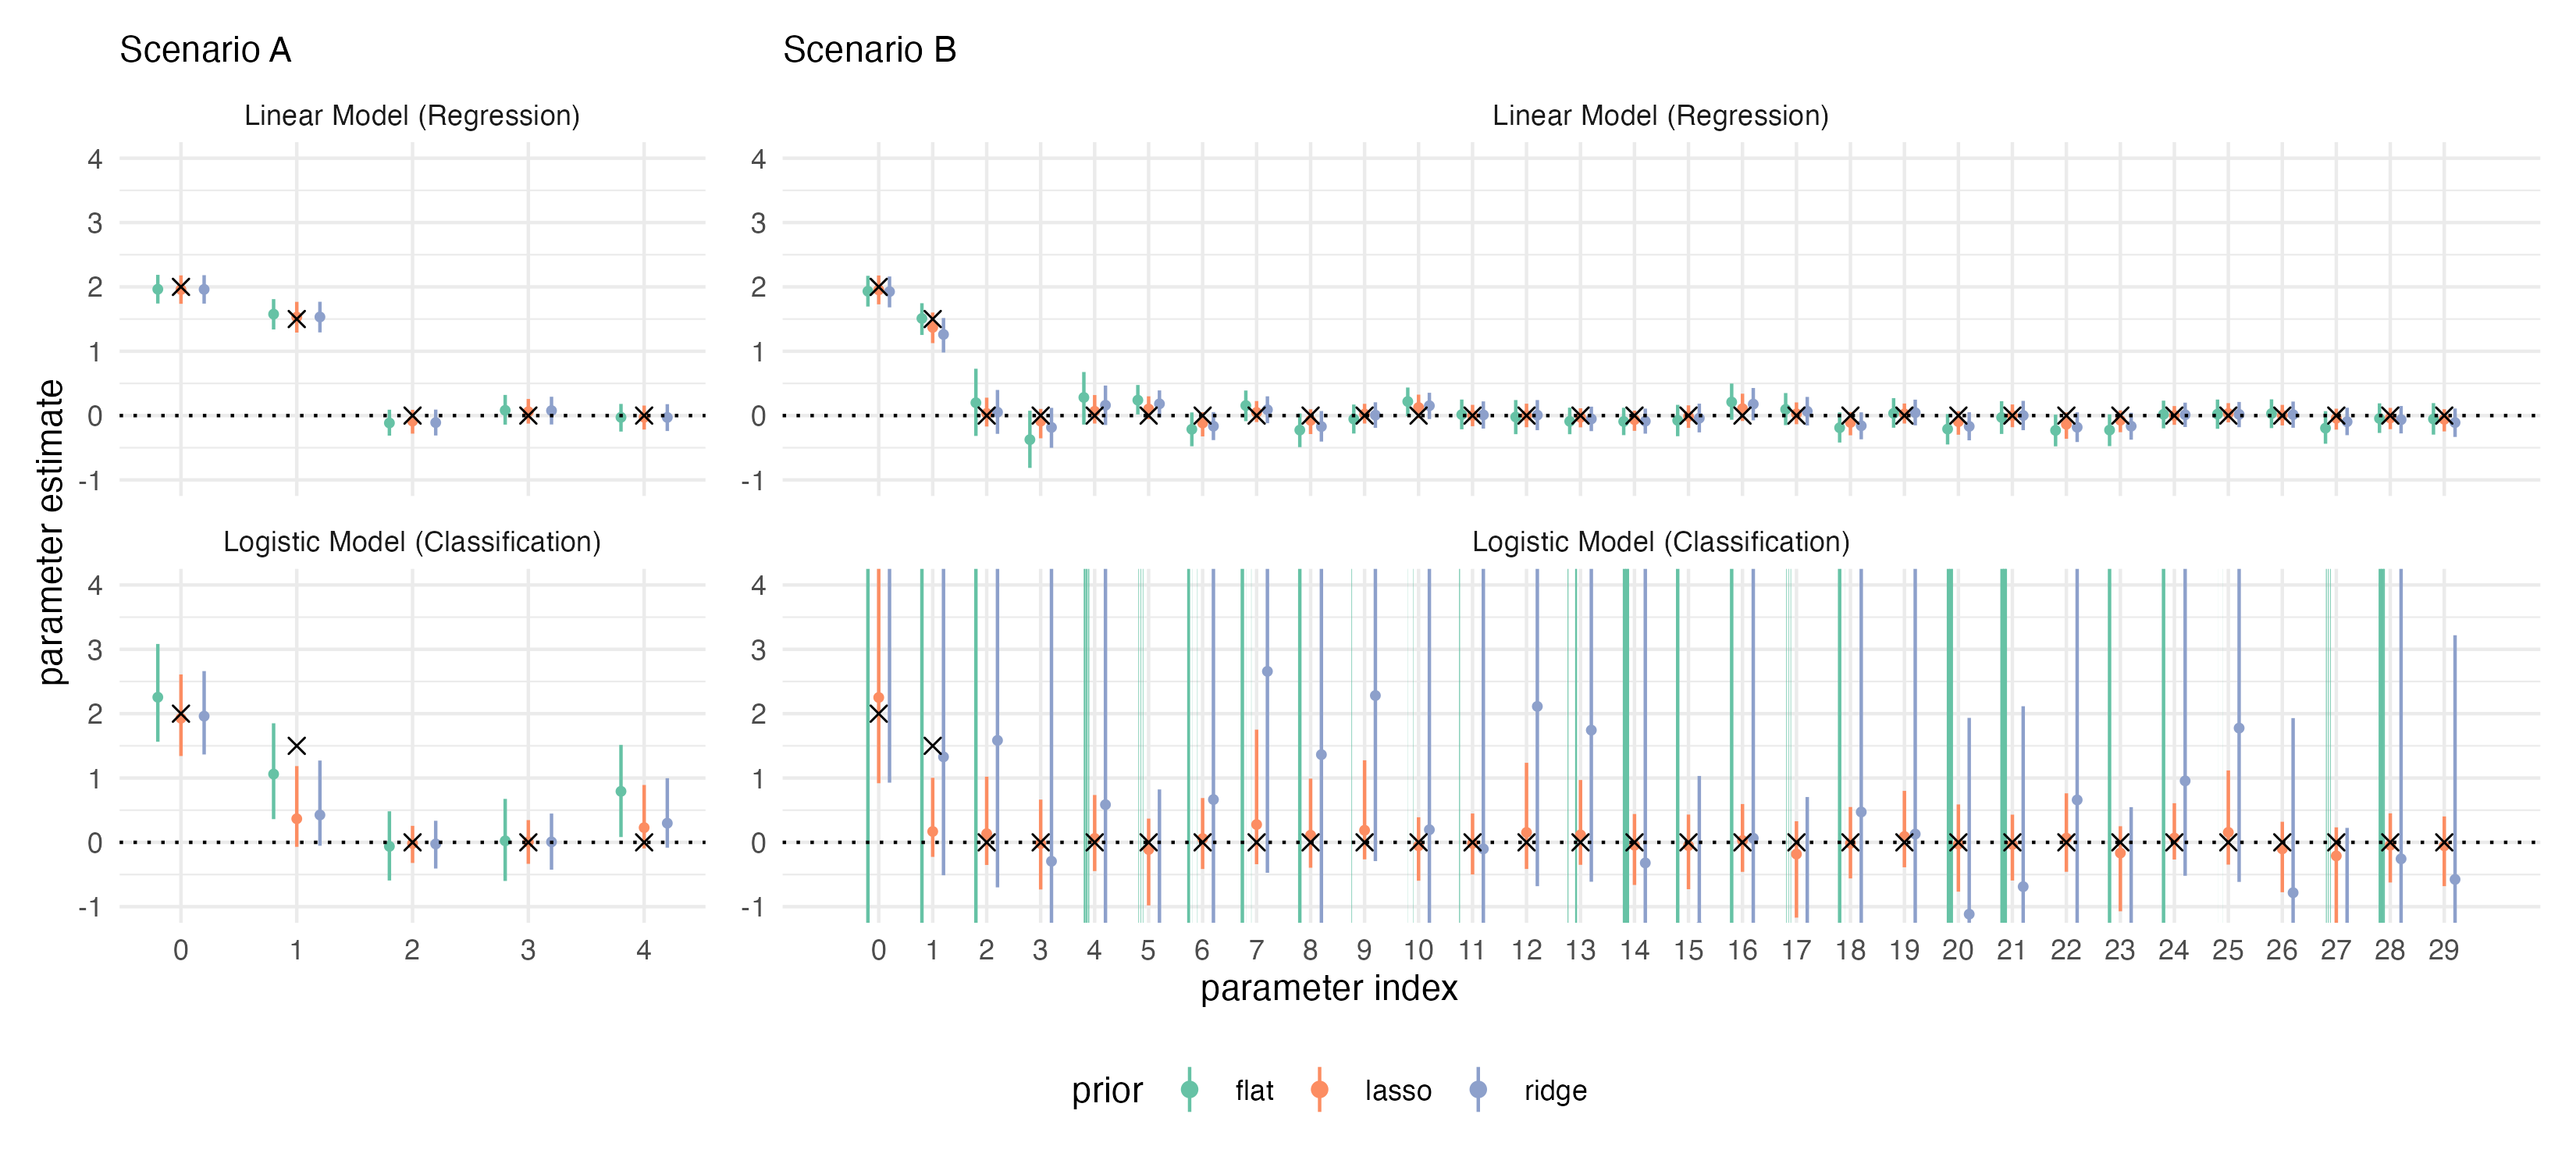
\includegraphics[width=\linewidth]{../figures/reg_all.png}
    \caption{Estimated model parameters with $95\%$ credibility interval (CI). The true parameters are notes as black crosses. Linear models produced more accurate estimates and smaller parameter CIs than logistic models. The necessity of regularization becomes apparent in scenario B, where the parameter estimates of the unregularized logistic model are very uncertain.}
    \label{fig:reg-params}
\end{figure}

\subsection{Performance of approximate inference algorithms in Bayesian regression}

In a second example, we compared the performance of LA and Metropolis-Hastings algorithms in Bayesian linear and logistic models.\\

We generate 1000 synthetic data sets with $n=100$:
\begin{equation*}
    \begin{aligned}
        &\bX \sim \Ncal(\bnull, \bI), \quad \btheta = (-0.5, 2, 1)\\
        &\text{linear: } \by \mid \btheta \sim \Ncal(\bX \btheta, \bI),\quad \text{logistic: } \by \mid \btheta \sim \text{Ber}(\sigma(\bX \btheta))
    \end{aligned}
\end{equation*}

We then fit one linear and one logistic model for each data set, using both LA and MCMC inference methods.
We assumed $\btheta \sim \Ncal(0, 10 \bI)$ and residual variance fixed at $\ssd = 10$. For LA, we used \texttt{r-INLA} with settings to default from INLA to simple LA.
For MCMC, we used the R-package \texttt{MCMCglmm} with settings specifically to use Metropolis Hastings, a relatively small sample size of 5000, a burnin periord of 500 and a thinning interval of 10. For both algorithms, we recorded the CPU runtime and the posterior parameter estimates and standard deviation.\\

Results for the linear and logistic model can be seen in \autoref{fig:approx-regr} and \autoref{fig:approx-class} respectively. In our experiment, LA was generally slower and thus more computationally expensive than MCMC methods, but this could also be mitigated by the specific implementation used in the experiment. In the case of the Bayesian linear model (\autoref{fig:approx-regr}), there is not much difference in the posterior parameter estimates, although LA leads to much higher standard deviation of parameters. In Logistic regression (\autoref{fig:approx-class}) on the other hand, LA outperforms MCMC in both parameter estimation and standard deviation.

\begin{figure}[htbp]
    \centering
    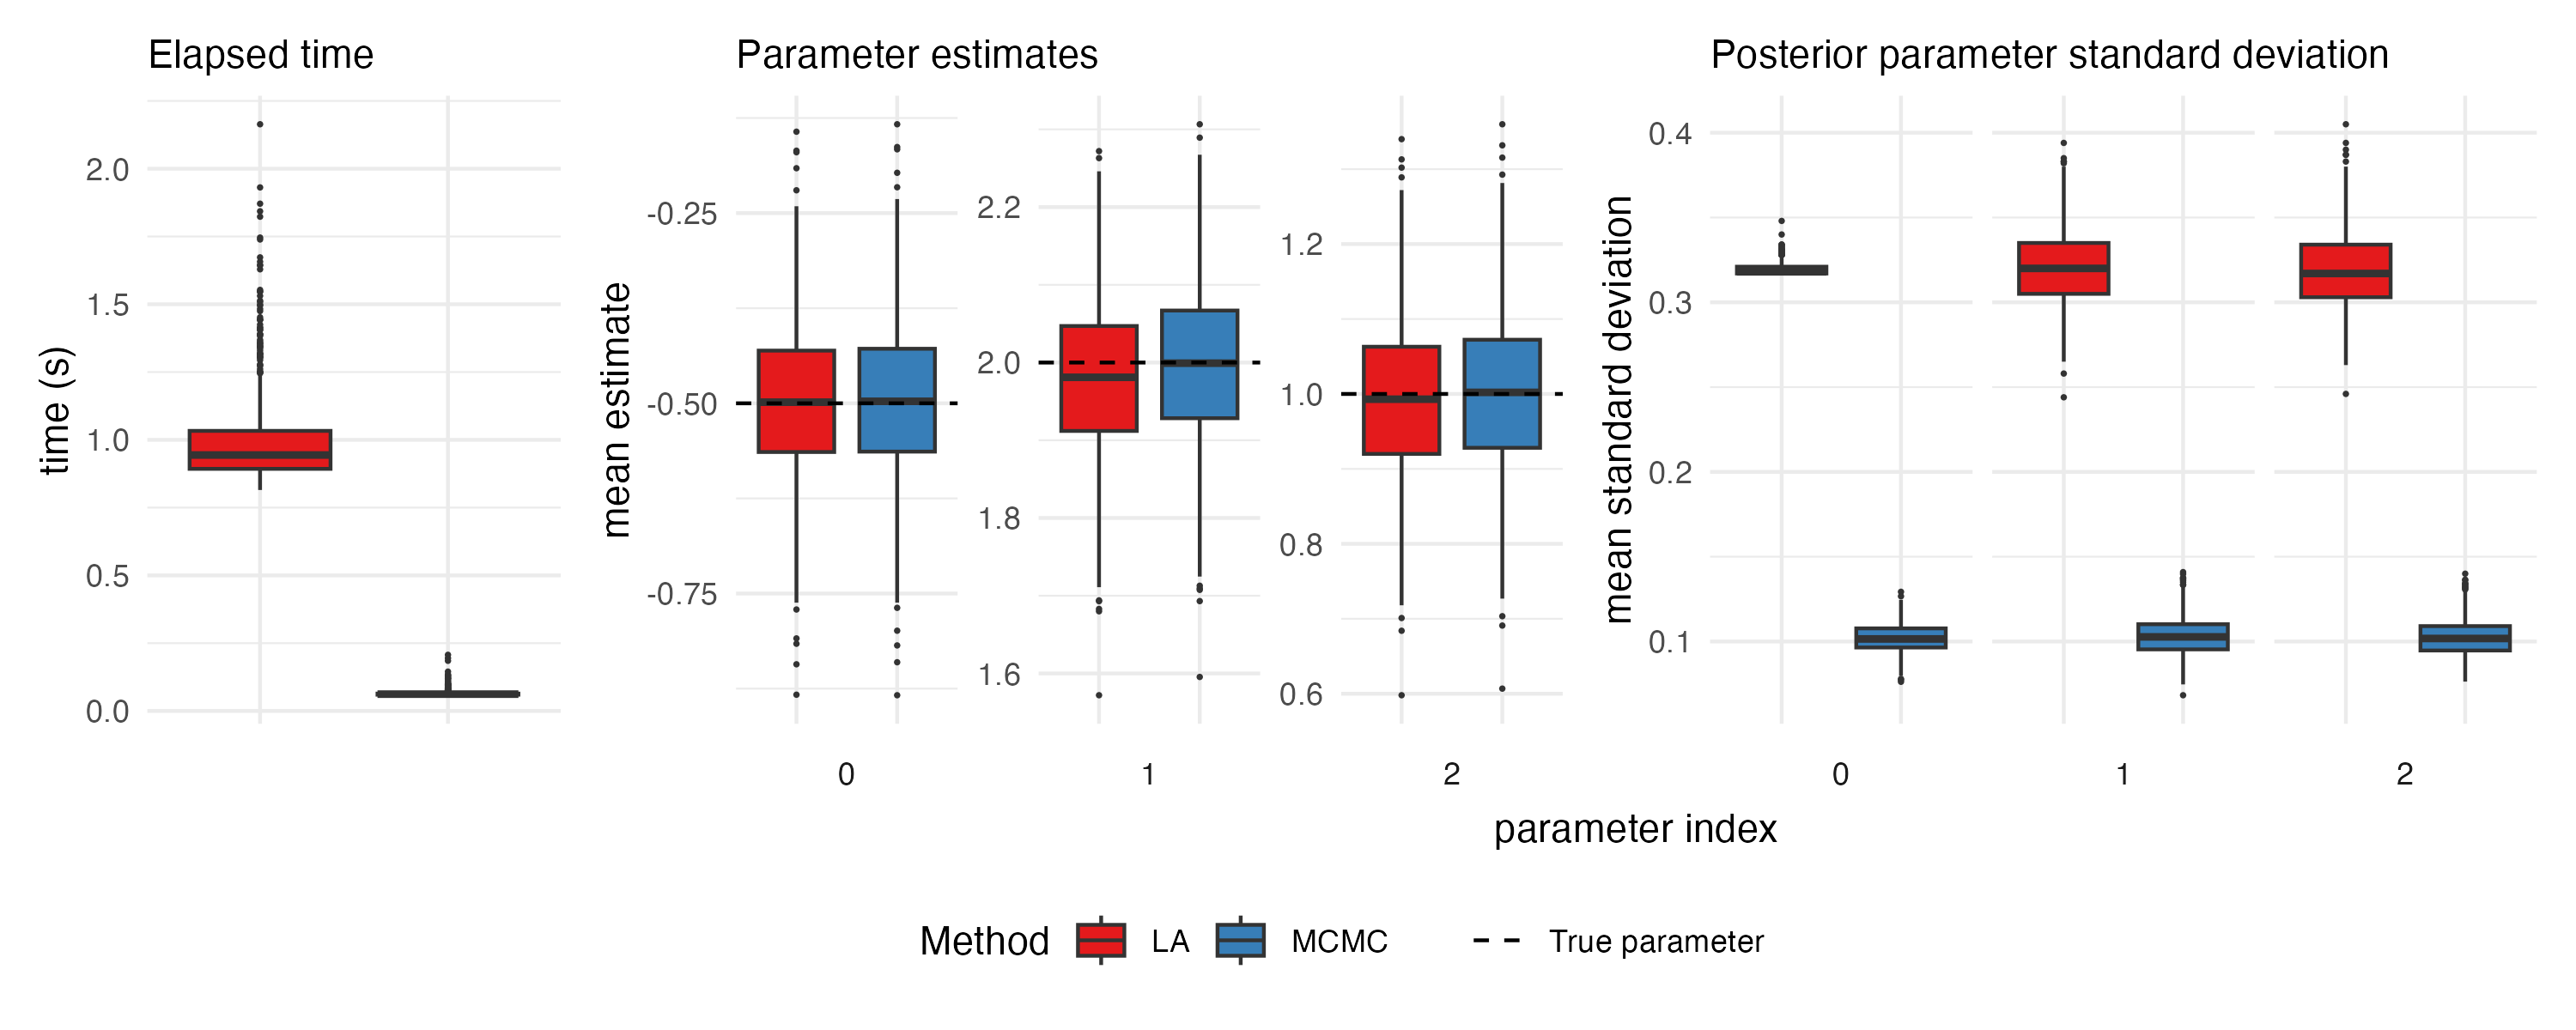
\includegraphics[width=\linewidth]{../figures/approx_regr.png}
    \caption{Linear regression: mean time, parameter estimates and standard deviation in LA and MCMC.}
    \label{fig:approx-regr}
\end{figure}

\begin{figure}[htbp]
    \centering
    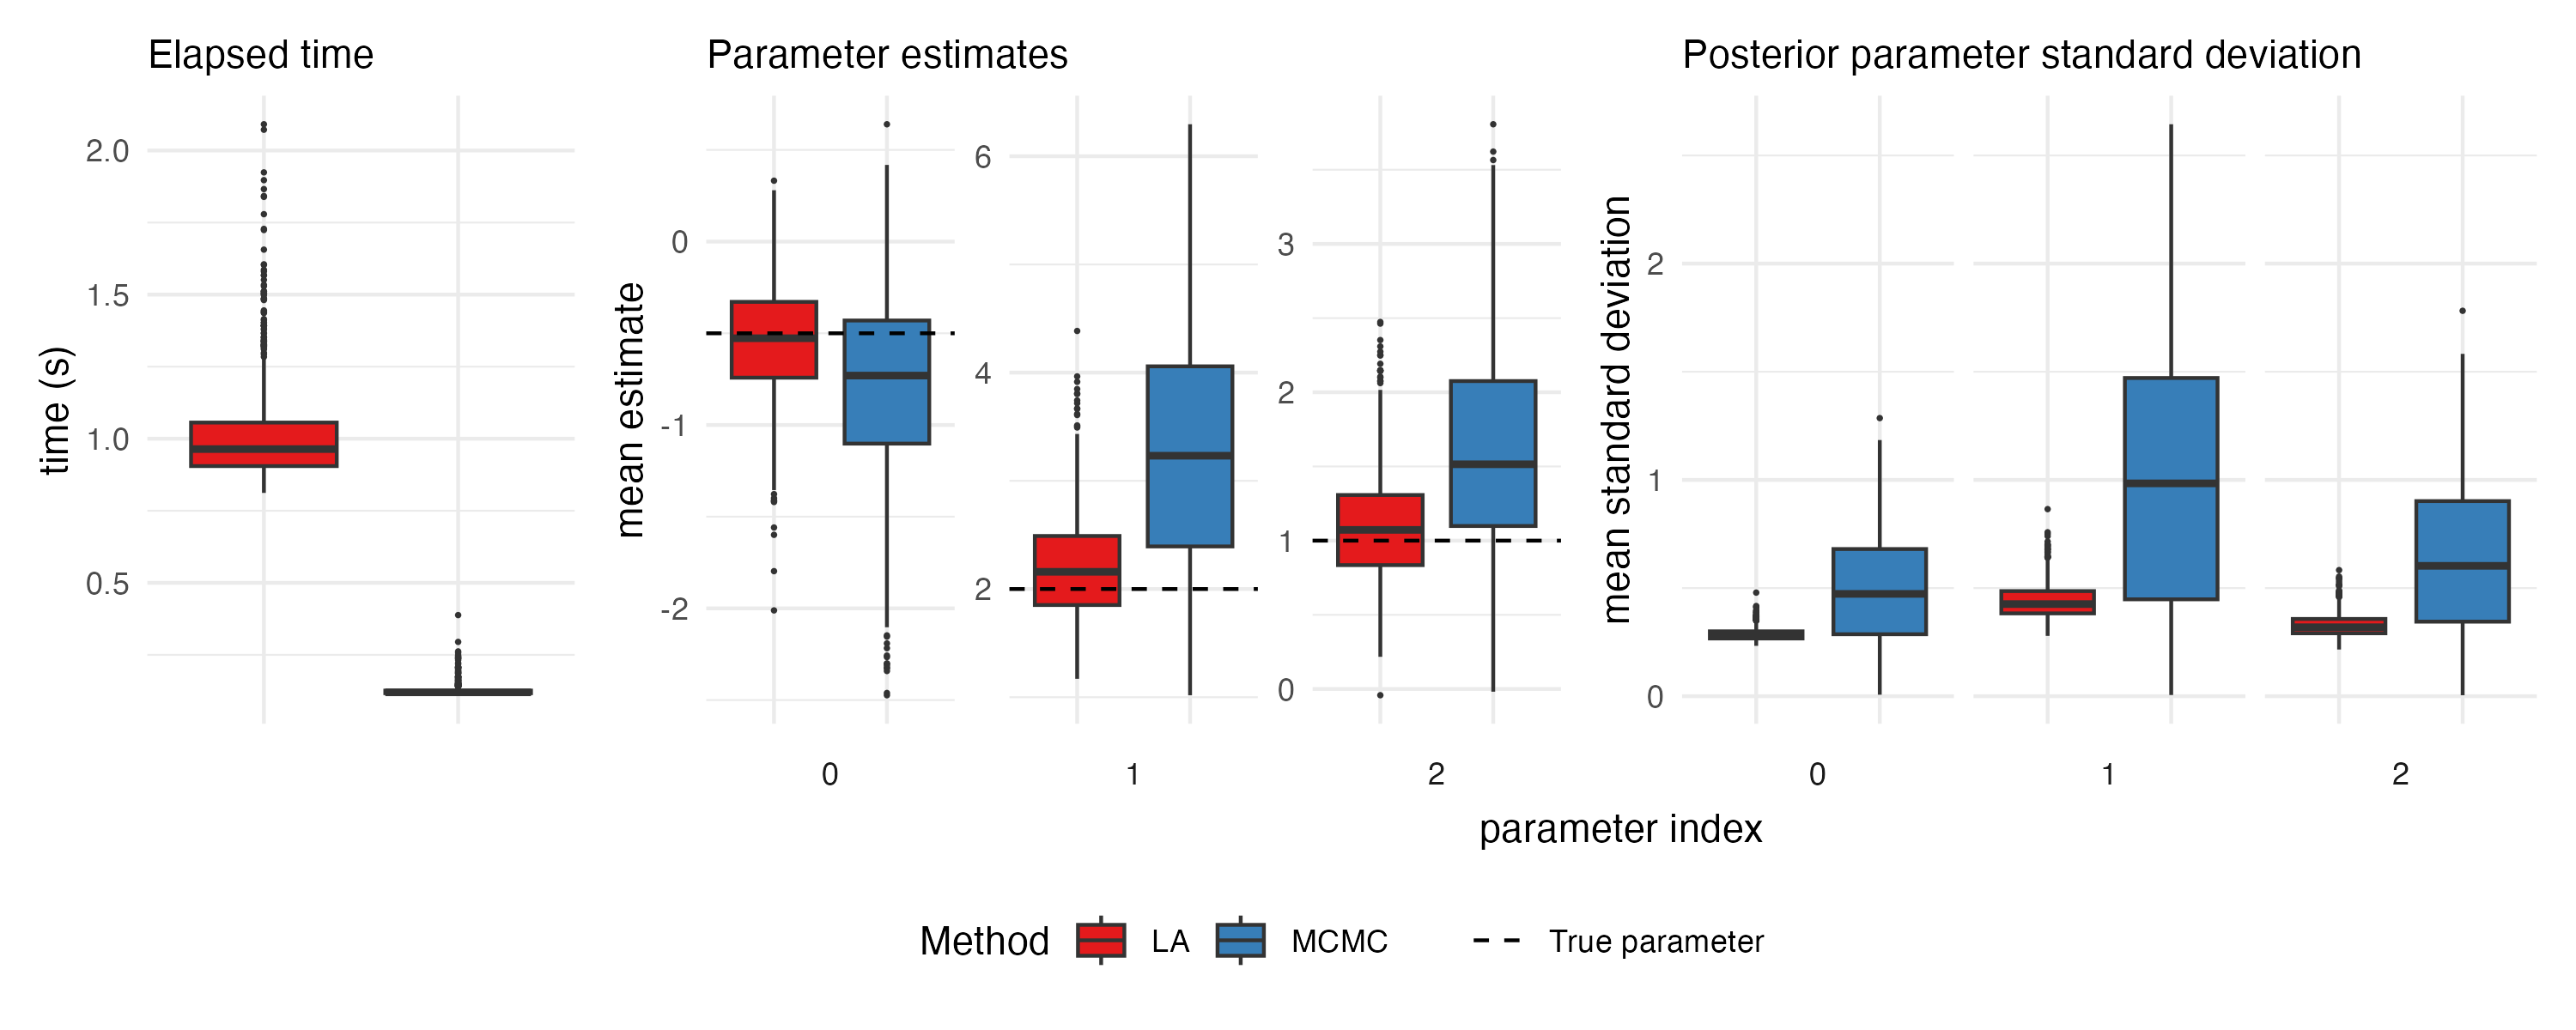
\includegraphics[width=\linewidth]{../figures/approx_class.png}
    \caption{Logistic regression: mean time, parameter estimates and standard deviation in LA and MCMC.}
    \label{fig:approx-class}
\end{figure}

